\section{Results}\label{sec:results}\label{sec:applications}
The results connect the quantitative comparisons to source-space interpretation. We first examine planar temporal maps, then a static slice and a sequence of static sections, followed by volumetric temporal data. Each comparison uses the same source features in P and R and reports the scalar connectivity exchanged for improved reference alignment. Temporal overviews, scalar profiles, and source views have distinct roles: they expose evolution, show connection thresholds, and locate features in the original domain, respectively.

% Declare the wide result figures before their discussion so that the
% two-column output routine can place them at the next page top.
\begin{figure*}[t]
\centering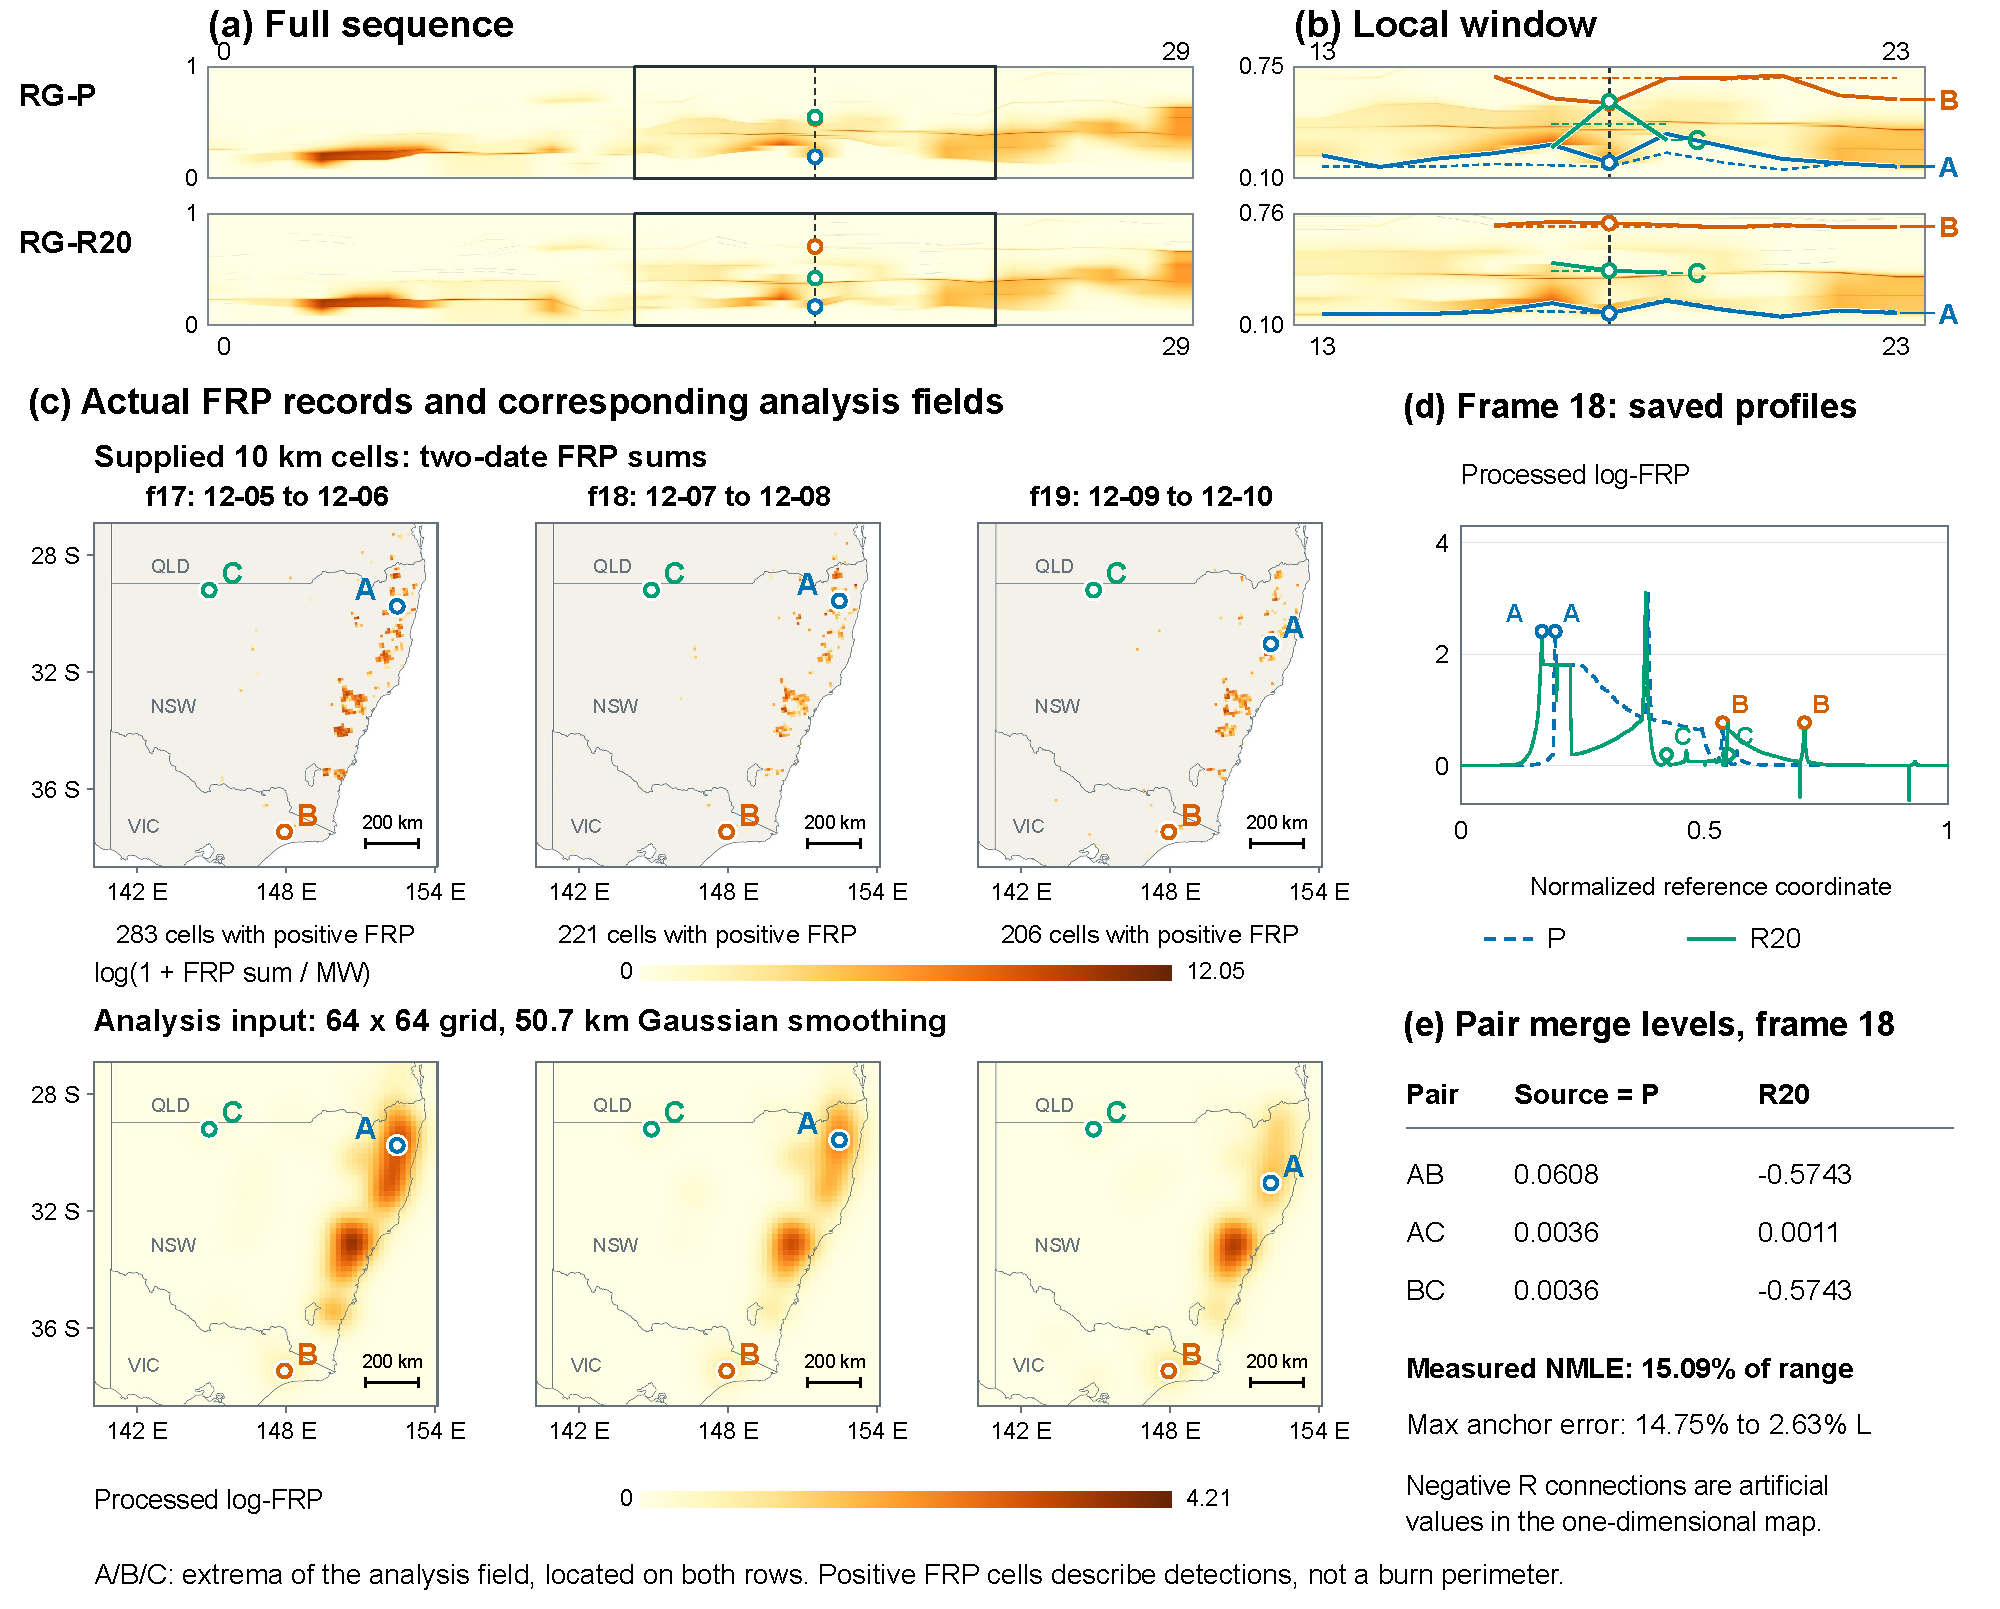
\includegraphics[width=\textwidth]{figures/Fig7.pdf}
\caption{Wildfires: RG-MTM-P/R over all 30 frames (a), with frames 13--23 enlarged (b). Panel (c), top: actual supplied 10-km FRP cell polygons for December 5--6, 7--8, and 9--10, 2019 (frames 17--19), on a geographic basemap~\cite{NaturalEarth:WildfireAdmin1}. Only cells with positive two-date FRP sums are colored; they indicate recorded fire activity rather than a burn perimeter. Bottom: the corresponding saved analysis fields, after aggregation onto a $64\times64$ grid (20.3-km cells), $\log(1+\mathrm{FRP}/\mathrm{MW})$, 50.7-km Gaussian smoothing, and the declared weak background. Both rows share the same extent, with geographic coordinates and 200-km scale bars. Tracks $A=3$, $B=48$, $C=52$ mark the same analysis extrema on both rows. Yellow--orange--brown uses fixed ranges 0--12.05 for supplied cells and 0--4.21 for processed fields and maps. Solid traces in (b) are anchors; dashed traces are references. At frame 18, relaxation reduces maximum displacement from 14.75\% to 2.63\% at 15.09\% actual NMLE. Panels (d)--(e) retain complete saved P/R scalar profiles and measured pair connection values. Negative connections are artificial map output, not negative observed FRP. This selected maximum-obstruction witness explains the mechanism; complete-sequence statistics and baseline panels are reported separately (Supplement S10). Temporal colour transitions use display interpolation only; saved frames, anchors, and evaluation samples are unchanged.}
\label{fig:fire_events}
\end{figure*}


\subsection{Two-Dimensional Data}\label{sec:results2d}
\subsubsection{Storms: Atmospheric Pressure}
Figure~\ref{fig:teaser} shows a separate hourly Storms visualization covering 1--31 December 1999 (744 hourly fields), using mean sea-level pressure anomalies relative to a centered 192-hour average. The analysis retains the fixed $49\times49$ grid, 250\,km smoothing and direction $d\approx(0.948,-0.319)$ estimated from the full sequence. The top R20 overview locates 2 December, 06:00--22:00 UTC and output positions $[0.10,0.42]$; its selected scalar columns are identical to R5. Five original-grid anomaly snapshots at 09:00, 10:00, 11:00, 13:00 and 18:00 locate the same processed extrema as the P/R1/R2/R5 maps. The fractions are eligibility controls $\kappa/\Delta_F$, not hard bounds on actual merge error. This visualization does not replace or extend the 118-frame half-day sequence used in the quantitative tables.

At 09:00, $A$ lies in the subtropical North Atlantic and $B$ near Iceland. Their projected references are $0.339L$ and $0.182L$, while P places them at $0.238L$ and $0.283L$, reversing their directional order. R5 restores that order with anchors $0.348L$ and $0.173L$. At 13:00, R1 restores the order of $A/C$; at 18:00, R2 restores $E/F$. The letter $E$ marks the computed minimum associated with the Anatol event context~\cite{Koepp:2023:TMTM}, rather than an independently validated physical track. The geographic position and directional reference of $A$ are unchanged between 09:00 and 10:00, but P moves its anchor by $0.110L$ as $B$ ceases to be an independent extracted extremum. R5 avoids this particular jump. The snapshots also explain why labels do not imply a continuous physical identity: $B$ is absent at 10:00 and 11:00, and the nearby extremum assigned track $C$ first appears at 12:00. Only features in the five displayed snapshots are marked in the lower maps. Supplement S8 records identities, source coordinates, the forward-prefix calculation and directly measured scalar costs.

In the separate 118-frame evaluation sequence, the 11 December 1999 case (Supplement S8) illustrates how geographic location and pressure connectivity interact. The source tree connects minima $A,B$ before the outside minimum $C$ joins, but the projection places $C$ between them. A preserving layout therefore moves at least one feature away from its reference. The certificate attributes $8.45\%$ of reference extent to this hierarchy obstruction. R admits the spatial order $A,C,B$ and places the marked tracks close to their source references. Across all five features at this time, maximum displacement decreases from 8.87\% for P to 0.83\% for R. The corresponding TMTM, ST-MTM, P, and R panels are retained in Supplement S8.

The improved alignment has an interpretable scalar price. The $A/B$ connection changes from approximately 994.1 to 1006.7\,hPa, while its connections to $C$ change from 1009.4 to 1006.7\,hPa. These are the pressure thresholds at which the displayed components connect. The worst-pair change is 12.558\,hPa, or 13.21\% actual NMLE; the complete-sequence mean is 1.47\%. Thus, the map exposes both the geographic order gained by relaxation and the pressure-connectivity detail exchanged for it. Supplement S8 provides the full frame-level measurements and analytical-versus-rendered costs.

% Declare the remaining planar figures before their discussion.
% Static planar figures are declared after the temporal comparisons.

\subsubsection{Wildfires: Fire Radiative Power}
The Wildfires sequence summarizes fire-radiative-power observations in 30 two-day intervals. Figure~\ref{fig:fire_events} shows stronger processed fire activity as orange--brown bands against the pale lower-valued background. Panel (c) distinguishes the supplied 10-km cell records from the smoothed fields used to construct the trees. The supplied polygons retain their actual geometry and sparse support: frames 17--19 contain 283, 221, and 206 cells with positive two-date sums. Coastlines, state boundaries, coordinates, and scale bars locate them in southeastern Australia. The lower row shows the unchanged analysis input, including the declared 50.7-km smoothing; its continuous regions do not establish continuous burning or a fire boundary. Both rows locate the same processed extrema $A$, $B$, and $C$, while both RG maps use the same fixed spatial reference. Supplement S10 retains the TMTM and ST-MTM panels with their native coordinates.

Frames 17--19 illustrate why this distinction matters. The projected location of feature $C$ stays fixed, yet its P band shifts upward at frame 18 and returns in the next observation. The R band stays close to the same reference through all three frames. The spatial snapshots and matching labels separate this layout-induced displacement from a change in the feature's observed reference position. The comparison concerns the same overlap-linked features and the same scalar observations.

At frame 18, the source hierarchy groups $A,B$ while the reference requests $A,C,B$. Relaxation reduces maximum displacement from 14.75\% to 2.63\% of reference extent. The connecting scalar profile changes as well: R lowers the $A/B$ barrier from 0.060800 to $-0.574262$ in processed log-FRP units. The grey-blue under-range colour shows this artificial connection level alongside the improved anchor alignment. The resulting actual NMLE is 15.09\%; the original fire observations remain nonnegative. Exact coordinates, orders, and costs are recorded in Supplement S7--S8.

At the selected frame, the complete profiles and pair table in Fig.~\ref{fig:fire_events}(d)--(e) make the scalar price explicit: the $A/B$ connection changes from 0.060800 in the source and P to $-0.574262$ in R20. This artificial negative connection yields the measured 0.635063 worst-pair change. The frame is a selected maximum-obstruction witness among the tracked three-feature conflicts, rather than a typical-case claim.
